\documentclass{beamer}

\setbeamertemplate{background canvas}[vertical shading][bottom=cyan!10,top=blue!10]

\usetheme{Warsaw}
\usefonttheme[onlysmall]{structurebold}

% pour le fichiers .pdf
\usepackage{graphicx}
\usepackage{color}
% pour les fichiers .png
% \usepackage{pgf,pgfarrows}
% \usepackage{pgf,pgfarrows}
\usepackage{amsmath,amssymb}
\usepackage[latin1]{inputenc}
\usepackage[T1]{fontenc}
\usepackage[french]{babel}
\usepackage{textcomp}
\setbeamercovered{dynamic}
\DeclareMathOperator*{\argmin}{argmin}

\title[Openturns developers training: agenda]{OpenTURNS developers training: agenda}
\author[R. Lebrun, copyright EADS 2011.]
{
  Trainer : R�gis LEBRUN\\ 
  EADS/IW/SE/AM\\
  regis.lebrun@eads.net
}



\date[March 22-25th 2011]
{
  Developers training \\

  \begin{center}
    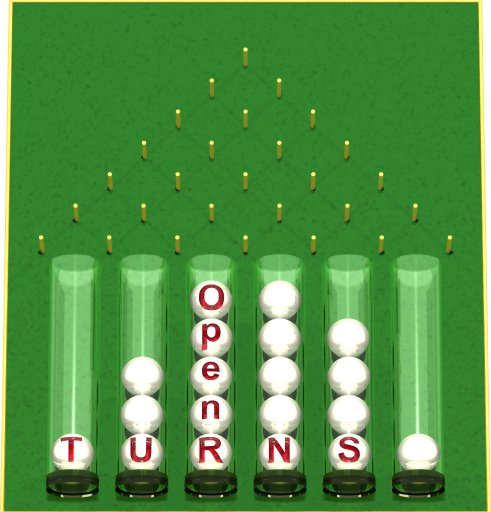
\includegraphics[height=2cm]{logoOT.jpg}
  \end{center}
}

\subject{OpenTURNS Developers Training}

% \part<presentation>{Corps de presentation}


\begin{document}

\frame{\titlepage}

% necessaire pour la table des matieres
\part{Main part}

%%%%%%%%%%%%%%%%%%%%%%%%%%%%% 
% Objective of the training %
%%%%%%%%%%%%%%%%%%%%%%%%%%%%% 
\begin{frame}
  \frametitle{The developers training}
  \begin{block}{Objectives}
    This 4 days training will give you the first elements to:
    \begin{itemize}
    \item Understand the OpenTURNS aim and architecture,
    \item Discover the coding rules, the development process and the associated infrastructure,
    \item Discover the OpenTURNS modules mechanism,
    \item Make your first steps in the OpenTURNS development by adding a new specialization of an existing concept both in the C++ library and the Python interface,
    \item Make your first steps in the OpenTURNS module development.
    \end{itemize}
  \end{block}
\end{frame}
%%%%%%%%%%%%%%%%%%%%%%%% 
% General organization %
%%%%%%%%%%%%%%%%%%%%%%%% 
\begin{frame}
  \frametitle{General organization}
  \begin{block}{Agenda}
    Each of these four days will be organized as follow:
    \begin{description}
    \item[10.00am] Welcome (coffee \& tea)
    \item[10.15am] Theory
    \item[12.30pm] Lunch
    \item[13.30pm] Theory or experimentation
    \item[15.30pm] Break (coffee \& tea)
    \item[15.45pm] Experimentation
    \item[18.00pm] End of the day
    \end{description}
  \end{block}
\end{frame}
%%%%%%%%%%%%%%%%%%%%%%%%%%%%%%%%%%%%%%%%%%%%%%% 
% Day 1: uncertainties, package, architecture %
%%%%%%%%%%%%%%%%%%%%%%%%%%%%%%%%%%%%%%%%%%%%%%% 
\begin{frame}
  \frametitle{Day by day...}
  \begin{block}{Day 1: uncertainties, OpenTURNS platform, architecture}
    \begin{itemize}
    \item Uncertainties: quick reminder on analysis, probability and statistics
    \item OpenTURNS platform: the global picture of OpenTURNS product and the website, short presentation of the development life-cycle.
    \item Architecture: the general organization of the product with some highlights on the key mechanisms and their implementation.
    \item Experimentation: basic manipulation of a numerical function and a probability distribution, navigation in the website (tickets, versioning system), exploration of examples en C++ and python.
    \end{itemize}
  \end{block}
\end{frame}
%%%%%%%%%%%%%%%%%%%%%%%%%%%%%%%%%%%%%%%%%%%%%%%%%%%%%%%%% 
% Day 2: development in OpenTURNS: the C++ library part %
%%%%%%%%%%%%%%%%%%%%%%%%%%%%%%%%%%%%%%%%%%%%%%%%%%%%%%%%% 
\begin{frame}
  \frametitle{Day by day...}
  \begin{block}{Day 2: development in the C++ library}
    \begin{itemize}
    \item The development infrastructure: some elements on autotools and CMake.
    \item The development process: use cases, architecture, C++ implementation, tests, documentation.
    \item Practical case: add a new distribution to the library.
    \end{itemize}
  \end{block}
\end{frame}
%%%%%%%%%%%%%%%%%%%%%%%%%%%%%%%%%%%%%%%%%%%%%%%%%%%% 
% Day 3: development in OpenTURNS: the python part %
%%%%%%%%%%%%%%%%%%%%%%%%%%%%%%%%%%%%%%%%%%%%%%%%%%%% 
\begin{frame}
  \frametitle{Day by day...}
  \begin{block}{Day 3: make the development visible in python}
    \begin{itemize}
    \item Interfacing C++ and Python using SWIG.
    \item The development process: SWIG interface, python modules, tests, documentation.
    \item Practical case: make the new distribution visible within the OpenTURNS Python module.
    \end{itemize}
  \end{block}
\end{frame}
%%%%%%%%%%%%%%%%%%%%%%%%%%%%%%%%%%%%%%%%%%%%%%%%%%%%%%%% 
% Day 4: development around OpenTURNS: create a module %
%%%%%%%%%%%%%%%%%%%%%%%%%%%%%%%%%%%%%%%%%%%%%%%%%%%%%%%% 
\begin{frame}
  \frametitle{Day by day...}
  \begin{block}{Day 4: create an OpenTURNS module}
    \begin{itemize}
    \item The concept of module, its standard structure.
    \item The key steps in the development of a module.
    \item How to install and use a module?
    \item Practical case: add a new distribution as a module.
    \end{itemize}
  \end{block}
\end{frame}
%%%%%%%%%%%%%% 
% Conclusion %
%%%%%%%%%%%%%% 
\begin{frame}
  \frametitle{Already a contributor}
  \begin{block}{You are a new OpenTURNs developer!}
    \begin{itemize}
    \item All the developments made during this training session will become part of OpenTURNS sooner or later, depending on their degree of maturity (quality ;) ?).
    \item The missing steps for a direct integration will be the testing phase, the validation phase and the documentation phase.
    \item The integration will be done using the EADS development branche (openturns/branches/lebrun).
    \end{itemize}
    Check the upcoming 0.14.0 release or a next release to see your work in action!
  \end{block}
\end{frame}
\end{document}
